\documentclass{stdlocal}
\begin{document}
\section{Evaluation and Results} % (fold)
\label{sec:evaluation}

% Due to the lack of an objective metric to measure the smoothing capability of a smoothing procedure, I omit a quantitative evaluation of the provided curve smoothing algorithm.
% The comparison to other smoothing algorithms would require a custom implementation.
% Instead to evaluate and validate the quality of the algorithm in the following are
% In table~\ref{tab:results-models}, a list of all used models for validating the quality of the curve smoothing algorithm is given.

A quantitative evaluation of this smoothing algorithm is problematic due to several reasons.
First, comparability to formerly established algorithms is not given since publications of such algorithms do usually not provide implementations in the form of publicly accessible code.
Own implementations of those algorithms would introduce subjectiveness and thus result in biased comparisons.
Also, implementing several algorithms for the objective of comparability would be beyond the scope of this work.

Secondly, there is no objective metric to measure smoothing capability of a smoothing procedure since the latter cannot be formulated as a general goal but is subject to specific requirements of the field it is implemented in.
Thus, the formulation of a general benchmark to which to compare this work is not feasible here.

Third, the generation of outcome cannot be automated since initially given curves need to be hand-drawn.
As such, it is impossible to recreate the drawing of one curve several times to generate comparable outcomes.
Instead, I aim for a strictly qualitative evaluation and validation of the algorithm.
Figures~\ref{fig:results-geodesics}, \ref{fig:results-no-scaling}, \ref{fig:results-half-scaling}, and \ref{fig:results-tweaked} show a compilation of example polyhedral surfaces on which I test the surface smoothing process.
Each figure depicts a different parameter combination for the discrete geodesic curvature stencil.
In table~\ref{tab:results-models} a list of all used models for validating the quality of the curve smoothing algorithm is given.
In order to tackle the problem of hand-drawn curves at least to some extent, I attempted to recreate similar curves on the same surface several times.
Each picture of the figures~\ref{fig:results-geodesics}, \ref{fig:results-no-scaling}, \ref{fig:results-half-scaling}, and \ref{fig:results-tweaked} gives an example of the curves I recreated.
The figure subscripts show the average number of iterations till convergence after which the curve does not further change for each example curve.

\begin{table}[H]
  \caption{%
    The table provides a list of models that are used as underlying polyhedral surfaces for surface mesh curves.
    Together with their name, also the count of their faces and topological vertices is given.
  }
  \label{tab:results-models}
  \centering
  \small
  \renewcommand{\arraystretch}{1.3}
  \begin{tabular}{lrr}
    \hline
    \textbf{Model} & \textbf{Vertices} & \textbf{Faces} \\
    \hline
    \hline
    \rowcolor{mathdefback}
    Torus & 3000 & 6000 \\
    Suzanne & 7958 & 15744 \\
    \rowcolor{mathdefback}
    Bunny & 34,835 & 69,666 \\
    Dragon & 50,000 & 100,000 \\
    \rowcolor{mathdefback}
    Julia Vase & 63,091 & 126,202 \\
    Spherical Harmonic & 44,852 & 89,700 \\
    \rowcolor{mathdefback}
    Sappho's Head & 140,864 & 281,724 \\
    Buddha & 14,351 & 28,736 \\
    \hline
  \end{tabular}
\end{table}


\begin{figure}
  \centering
  \begin{subfigure}[b]{0.24\linewidth}
    \centering
    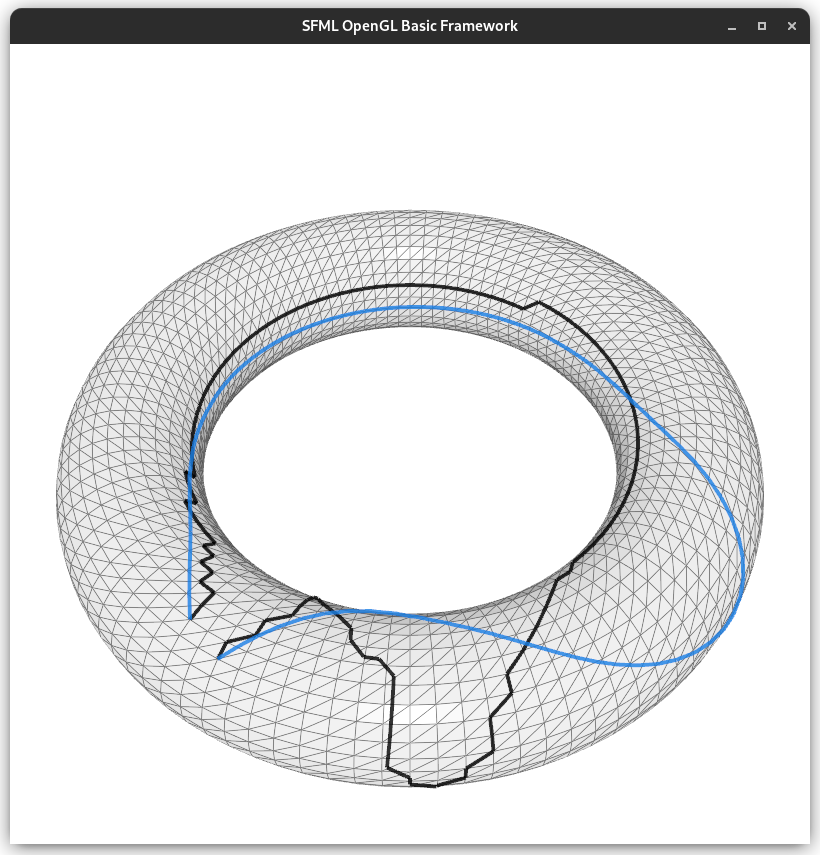
\includegraphics[width=\linewidth,trim={15px 20 15 50},clip]{images/torus-geodesic-1.png}
    \caption{$\sim 7500$}
  \end{subfigure}
  \begin{subfigure}[b]{0.24\linewidth}
    \centering
    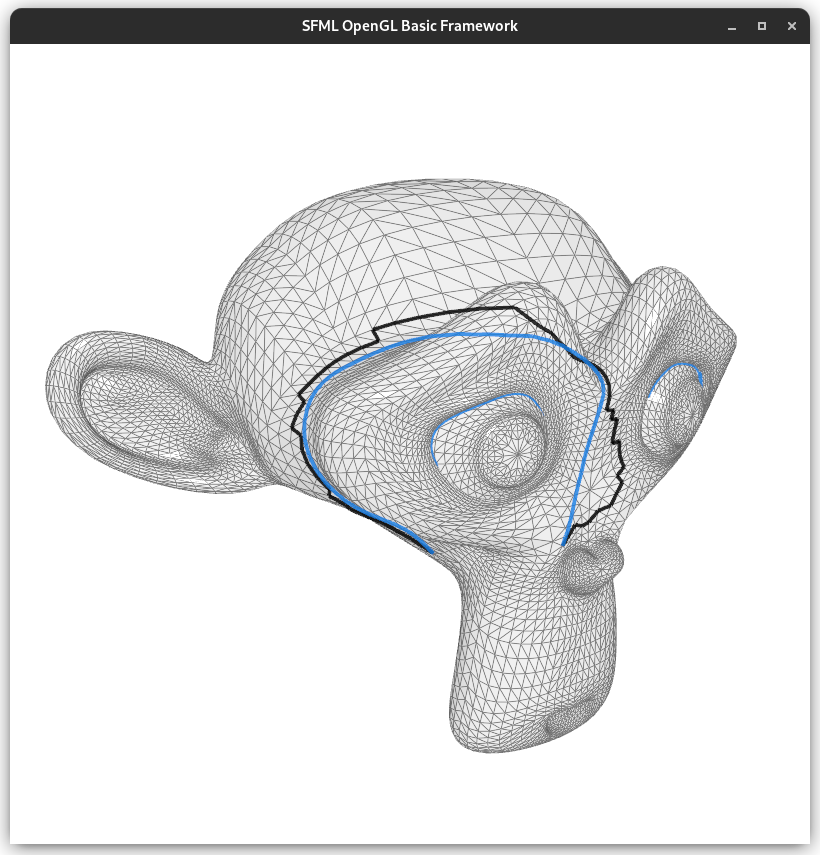
\includegraphics[width=\linewidth,trim={15px 20 15 50},clip]{images/suzanne-geodesic-1.png}
    \caption{$\sim 500$}
  \end{subfigure}
  \begin{subfigure}[b]{0.24\linewidth}
    \centering
    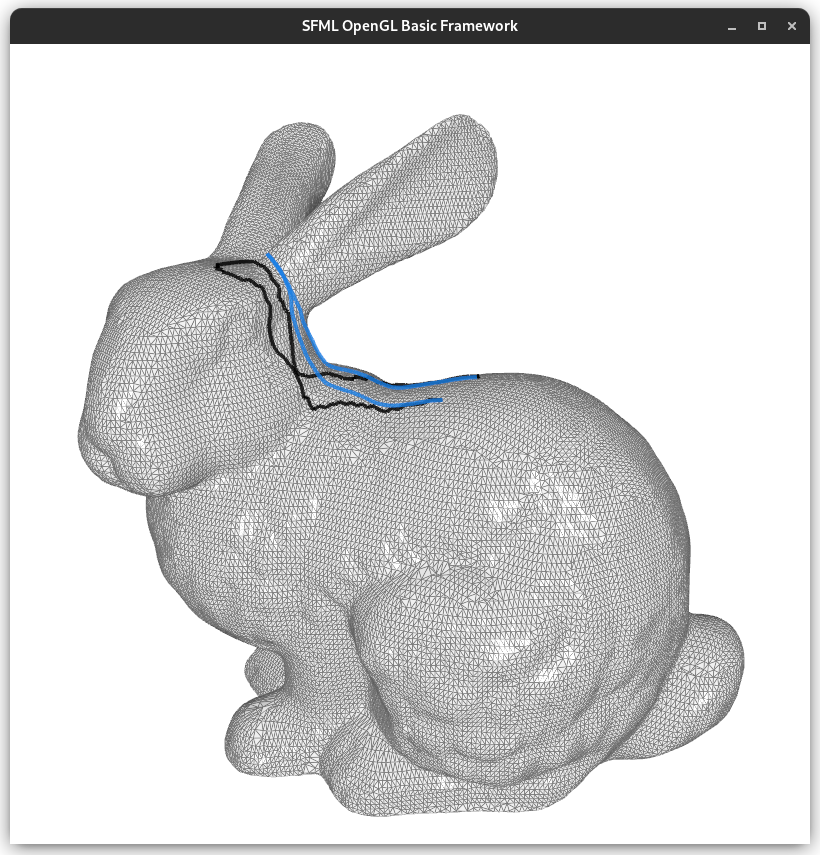
\includegraphics[width=\linewidth,trim={15px 20 15 50},clip]{images/bunny-geodesic-1.png}
    \caption{$\sim 4000$}
  \end{subfigure}
  \begin{subfigure}[b]{0.24\linewidth}
    \centering
    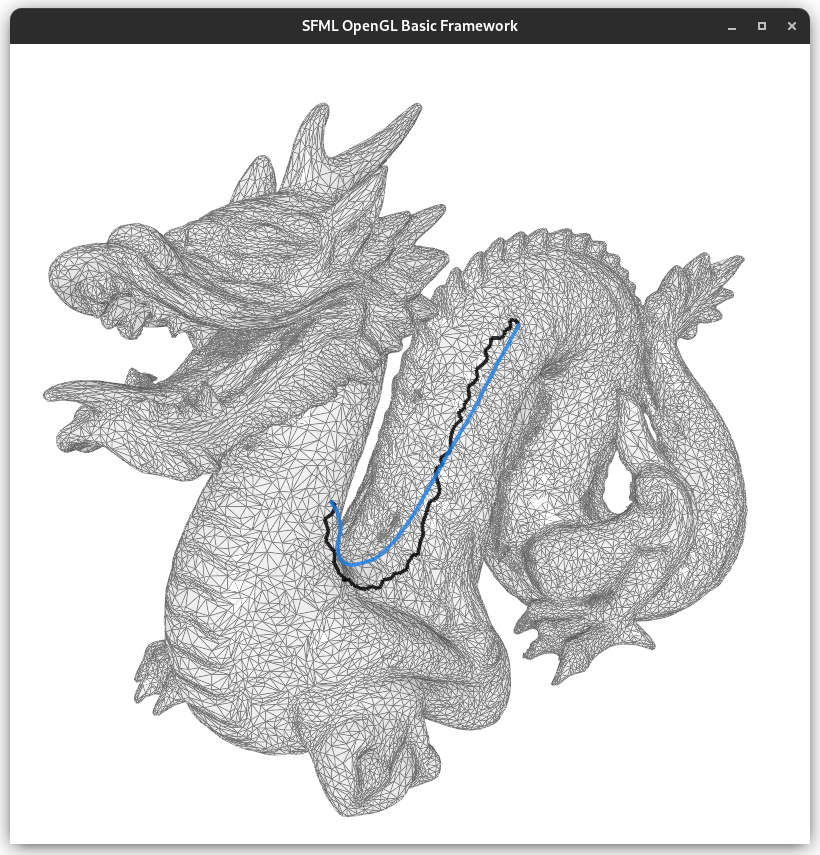
\includegraphics[width=\linewidth,trim={15px 20 15 50},clip]{images/dragon-geodesic-1.png}
    \caption{$\sim 2000$}
  \end{subfigure}

  \begin{subfigure}[b]{0.24\linewidth}
    \centering
    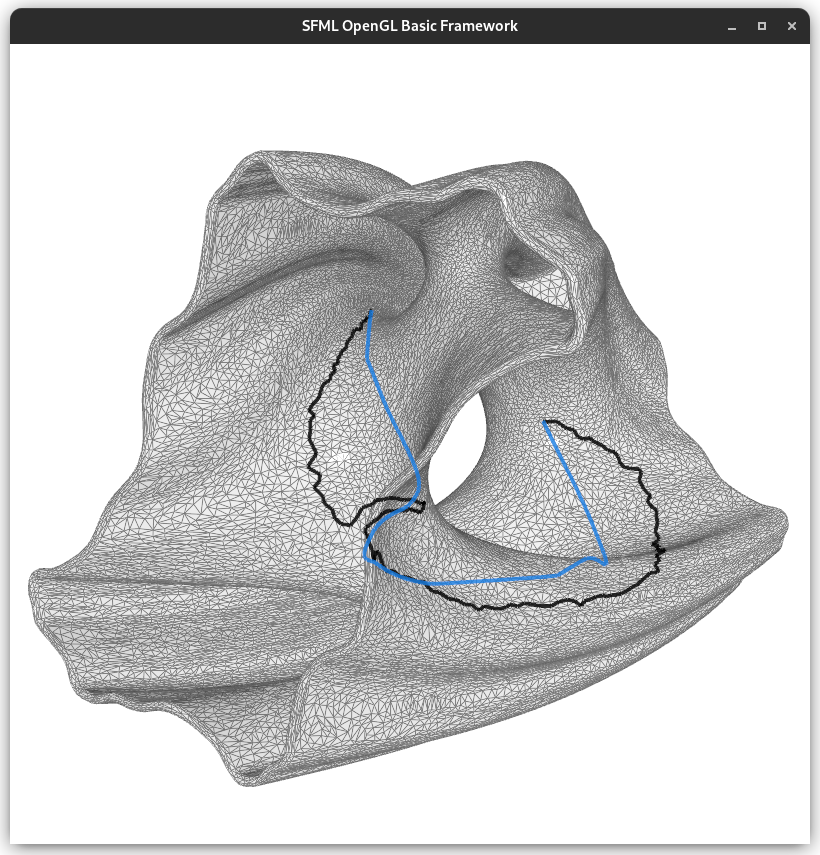
\includegraphics[width=\linewidth,trim={15px 20 15 50},clip]{images/julia-geodesic-1.png}
    \caption{$\sim 2000$}
  \end{subfigure}
  \begin{subfigure}[b]{0.24\linewidth}
    \centering
    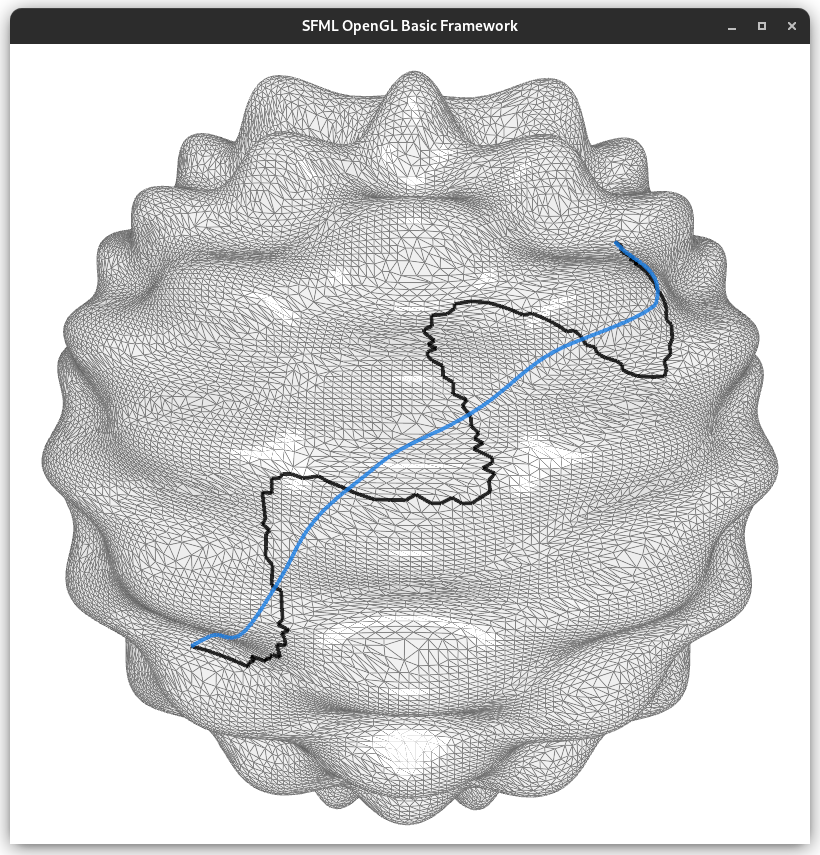
\includegraphics[width=\linewidth,trim={15px 20 15 50},clip]{images/harmonic-geodesic-1.png}
    \caption{$\sim 2000$}
  \end{subfigure}
  \begin{subfigure}[b]{0.24\linewidth}
    \centering
    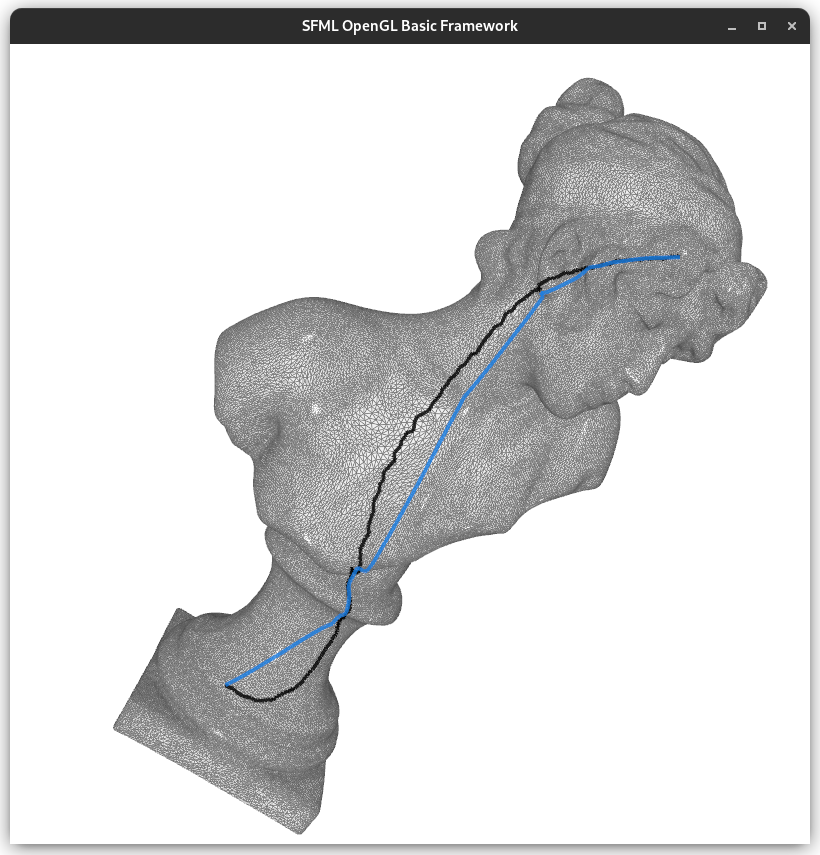
\includegraphics[width=\linewidth,trim={15px 20 15 50},clip]{images/sappho-geodesic-1.png}
    \caption{$\sim 5000$}
  \end{subfigure}
  \begin{subfigure}[b]{0.24\linewidth}
    \centering
    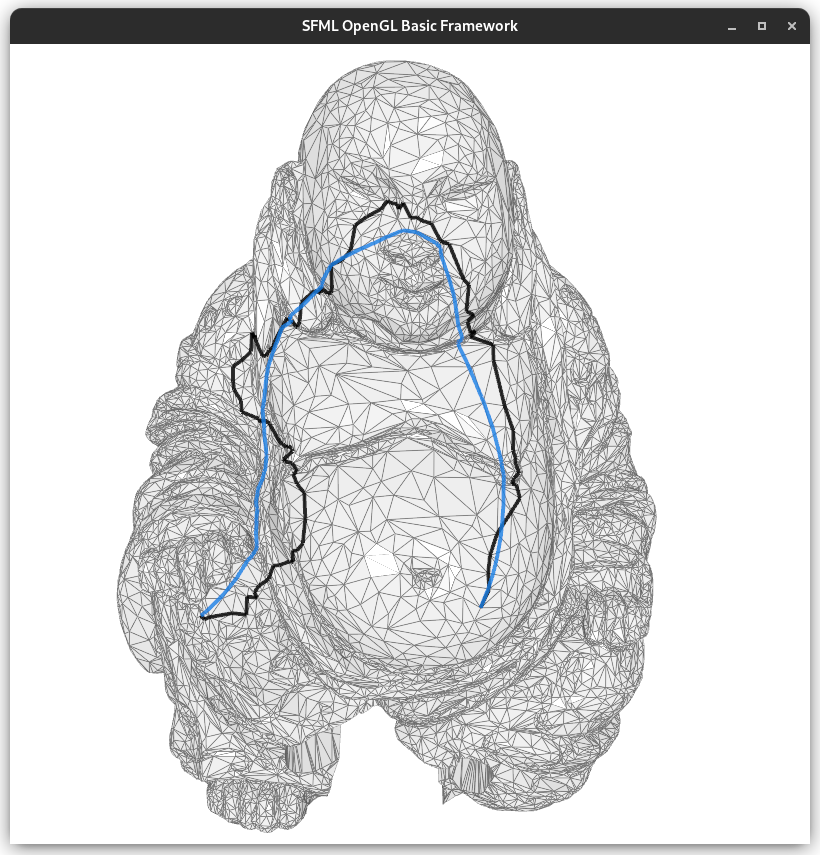
\includegraphics[width=\linewidth,trim={15px 20 15 50},clip]{images/buddha-geodesic-1.png}
    \caption{$\sim 1500$}
  \end{subfigure}
  \caption[Qualitative Results for Geodesics Generation]{%
    \textbf{Qualitative Results for Geodesics Generation}\\
    The images show the polyhedral surfaces of the selection of models from table~\ref{tab:results-models}.
    The black curve is the initially given surface mesh curve that the smoothing algorithm transformed into the blue curve.
    The scaling value of the desired geodesic curvature stencil has been set to $0$ to allow for the generation of locally shortest geodesics.
    All images are labeled by the average count of iterations till convergence is reached for initial curves that are close to the depicted one.
  }
  \label{fig:results-geodesics}
\end{figure}

\begin{figure}
  \centering
  \begin{subfigure}[b]{0.24\linewidth}
    \centering
    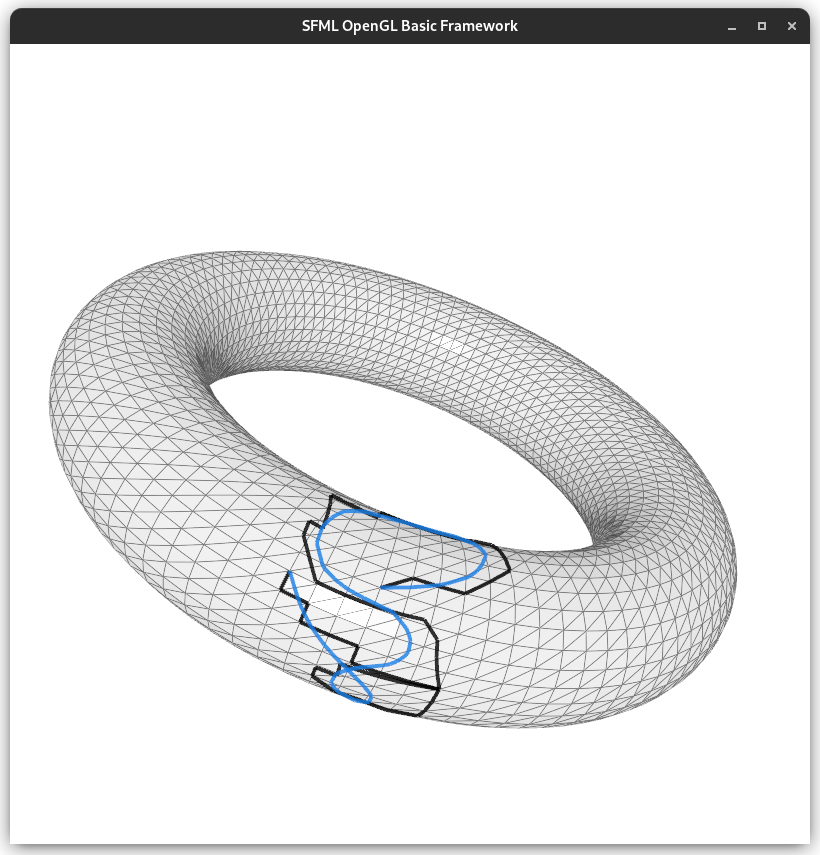
\includegraphics[width=\linewidth,trim={15px 20 15 50},clip]{images/torus-smooth-1.png}
    \caption{$\sim 500$}
  \end{subfigure}
  \begin{subfigure}[b]{0.24\linewidth}
    \centering
    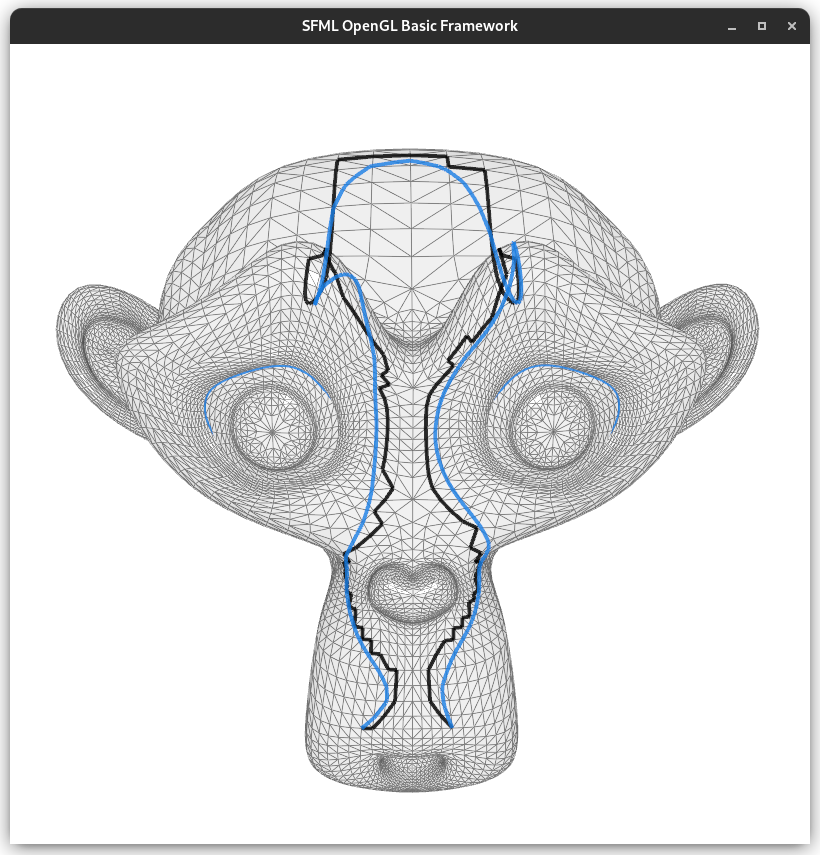
\includegraphics[width=\linewidth,trim={15px 20 15 50},clip]{images/suzanne-smooth-1.png}
    \caption{$\sim 500$}
  \end{subfigure}
  \begin{subfigure}[b]{0.24\linewidth}
    \centering
    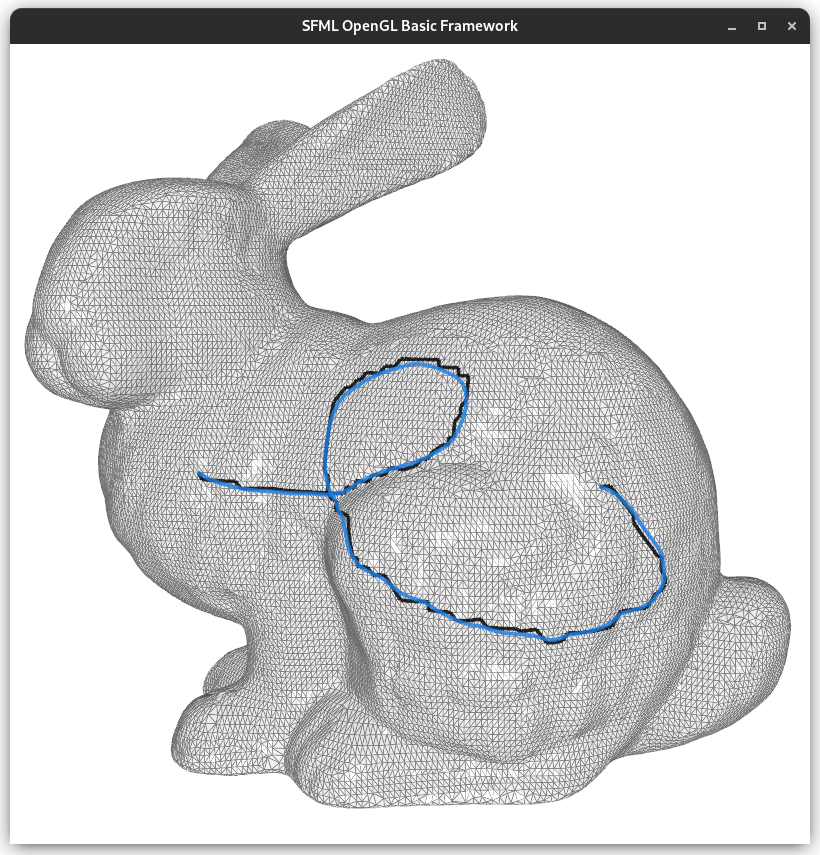
\includegraphics[width=\linewidth,trim={15px 20 15 50},clip]{images/bunny-smooth-1.png}
    \caption{$\sim 1000$}
  \end{subfigure}
  \begin{subfigure}[b]{0.24\linewidth}
    \centering
    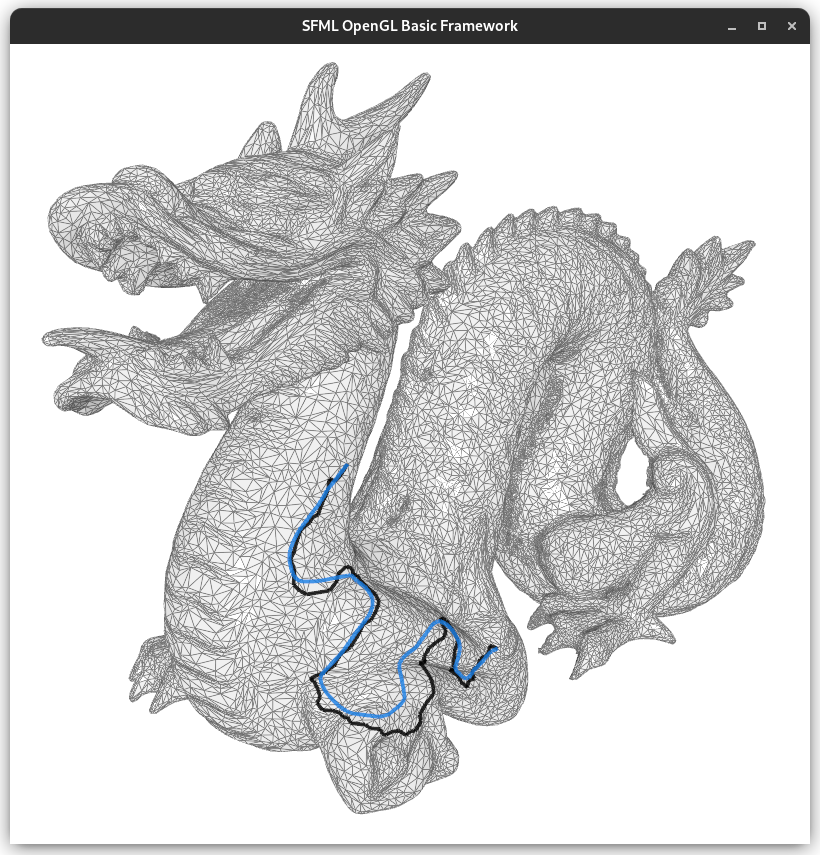
\includegraphics[width=\linewidth,trim={15px 20 15 50},clip]{images/dragon-smooth-1.png}
    \caption{$\sim 1000$}
  \end{subfigure}

  \begin{subfigure}[b]{0.24\linewidth}
    \centering
    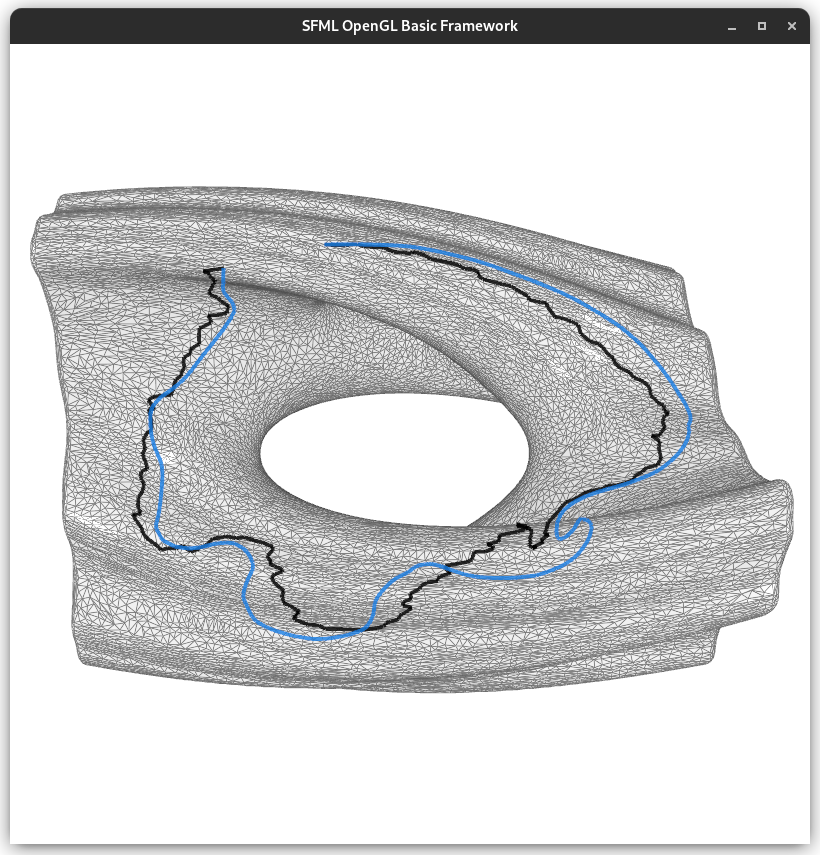
\includegraphics[width=\linewidth,trim={15px 20 15 50},clip]{images/julia-smooth-1.png}
    \caption{$\sim 1500$}
  \end{subfigure}
  \begin{subfigure}[b]{0.24\linewidth}
    \centering
    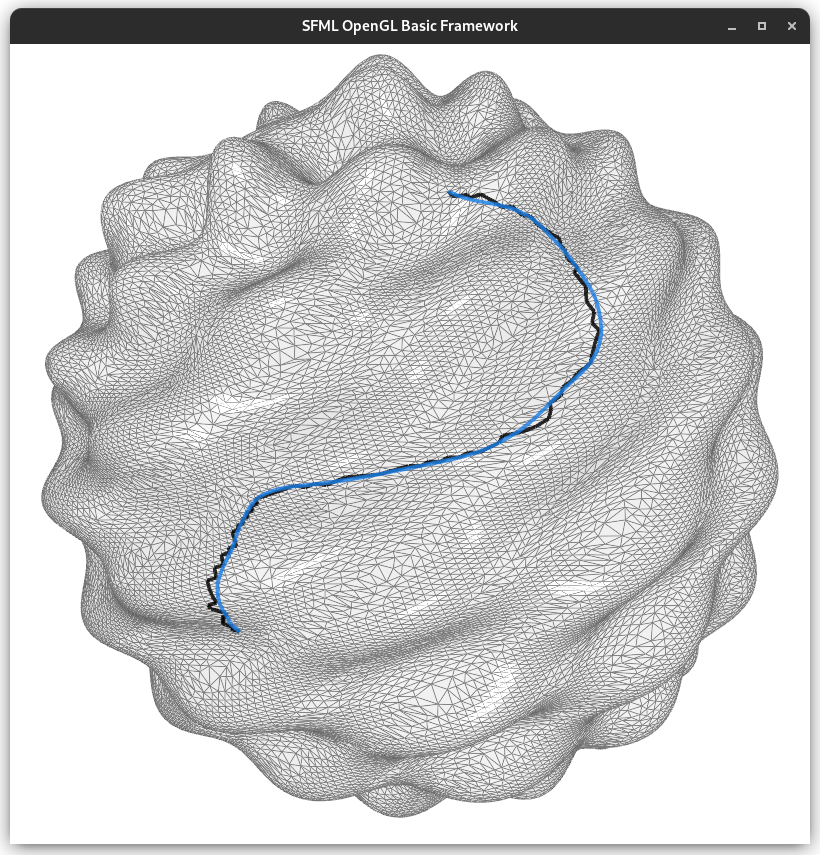
\includegraphics[width=\linewidth,trim={15px 20 15 50},clip]{images/harmonic-smooth-1.png}
    \caption{$\sim 2000$}
  \end{subfigure}
  \begin{subfigure}[b]{0.24\linewidth}
    \centering
    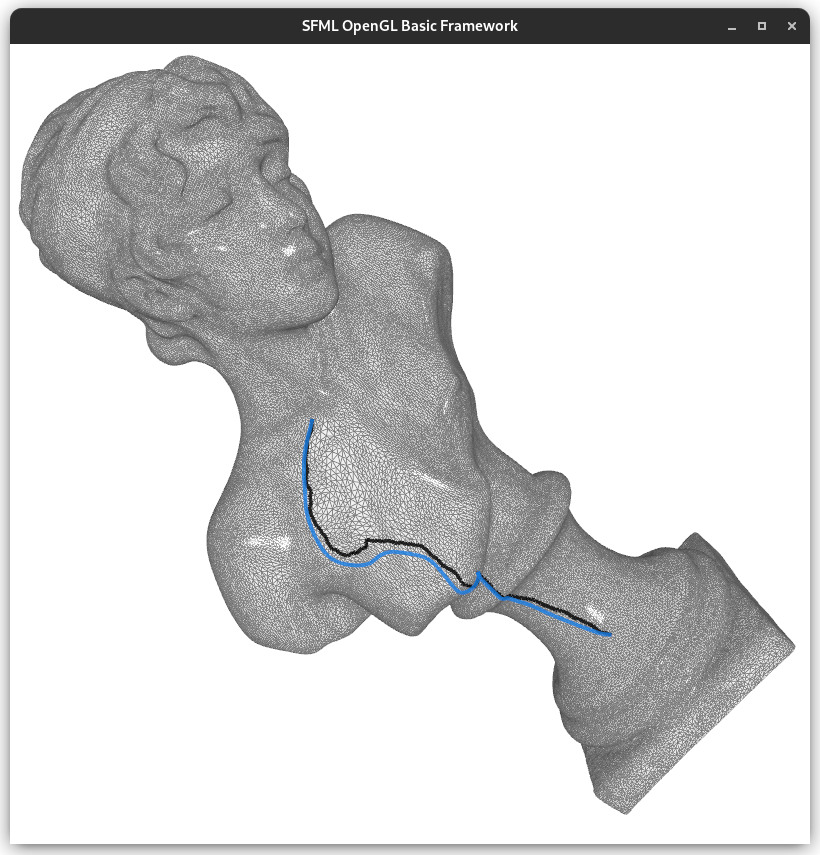
\includegraphics[width=\linewidth,trim={15px 20 15 50},clip]{images/sappho-smooth-1.png}
    \caption{$\sim 2000$}
  \end{subfigure}
  \begin{subfigure}[b]{0.24\linewidth}
    \centering
    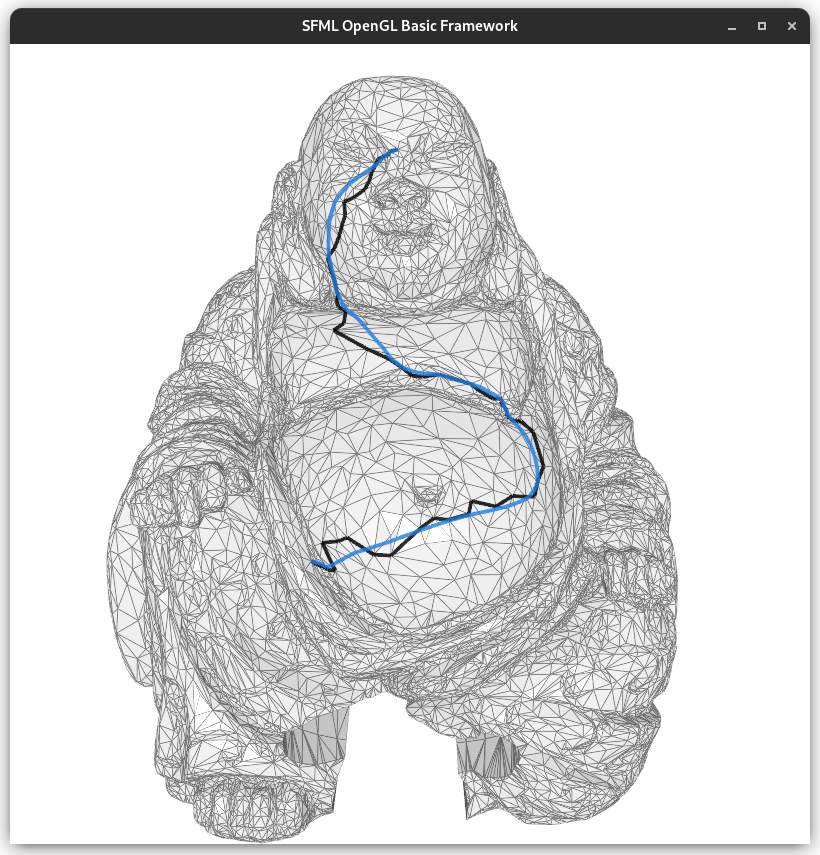
\includegraphics[width=\linewidth,trim={15px 20 15 50},clip]{images/buddha-smooth-1.png}
    \caption{$\sim 300$}
  \end{subfigure}
  \caption[Qualitative Results for Smoothing with no Scaling and Ten-Fold Stencil]{%
    \textbf{Qualitative Results for Smoothing with no Scaling and Ten-Fold Stencil}\\
    The images show the polyhedral surfaces of the selection of models from table~\ref{tab:results-models}.
    The black curve is the initially given surface mesh curve that the smoothing algorithm transformed into the blue curve.
    The scaling value of the initialization has been set to $1$ and the desired geodesic curvature stencil is applied $10$ times.
    All images are labeled by the average count of iterations till convergence is reached for initial curves that are close to the depicted one.
  }
  \label{fig:results-no-scaling}
\end{figure}

\begin{figure}
  \centering
  \begin{subfigure}[b]{0.24\linewidth}
    \centering
    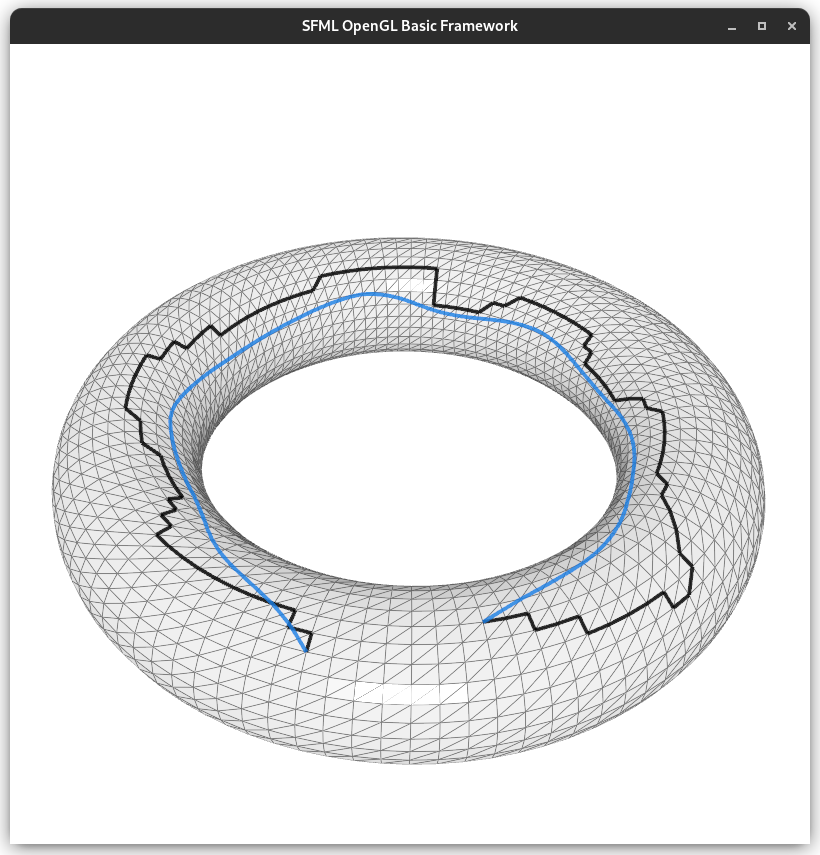
\includegraphics[width=\linewidth,trim={15px 20 15 50},clip]{images/torus-smooth-0.5.png}
    \caption{$\sim 1200$}
  \end{subfigure}
  \begin{subfigure}[b]{0.24\linewidth}
    \centering
    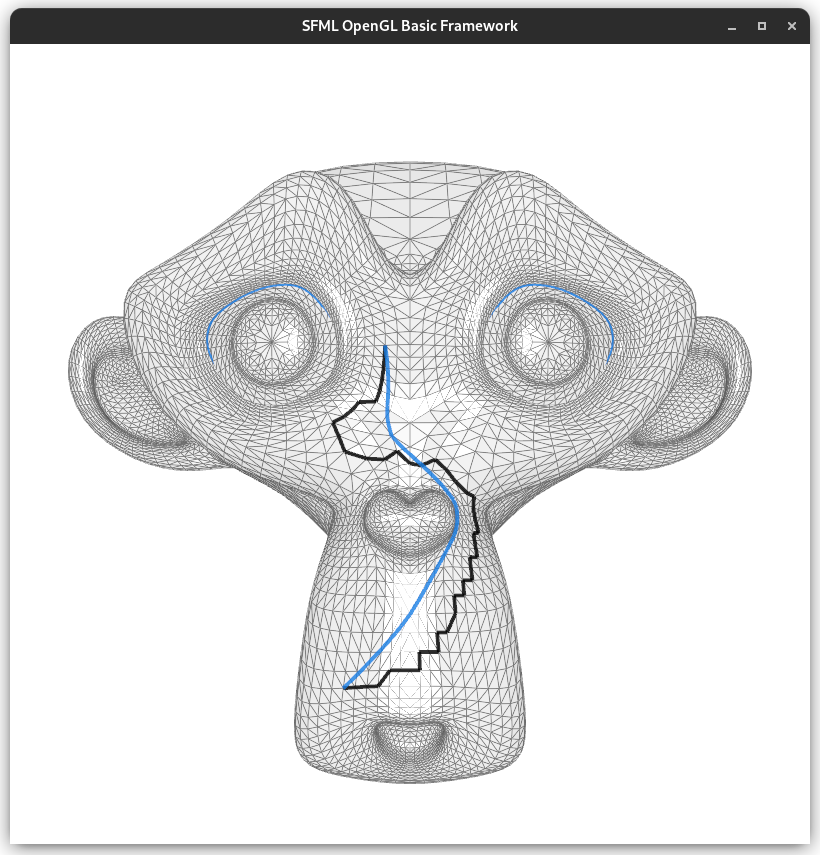
\includegraphics[width=\linewidth,trim={15px 20 15 50},clip]{images/suzanne-smooth-0.5.png}
    \caption{$\sim 1000$}
  \end{subfigure}
  \begin{subfigure}[b]{0.24\linewidth}
    \centering
    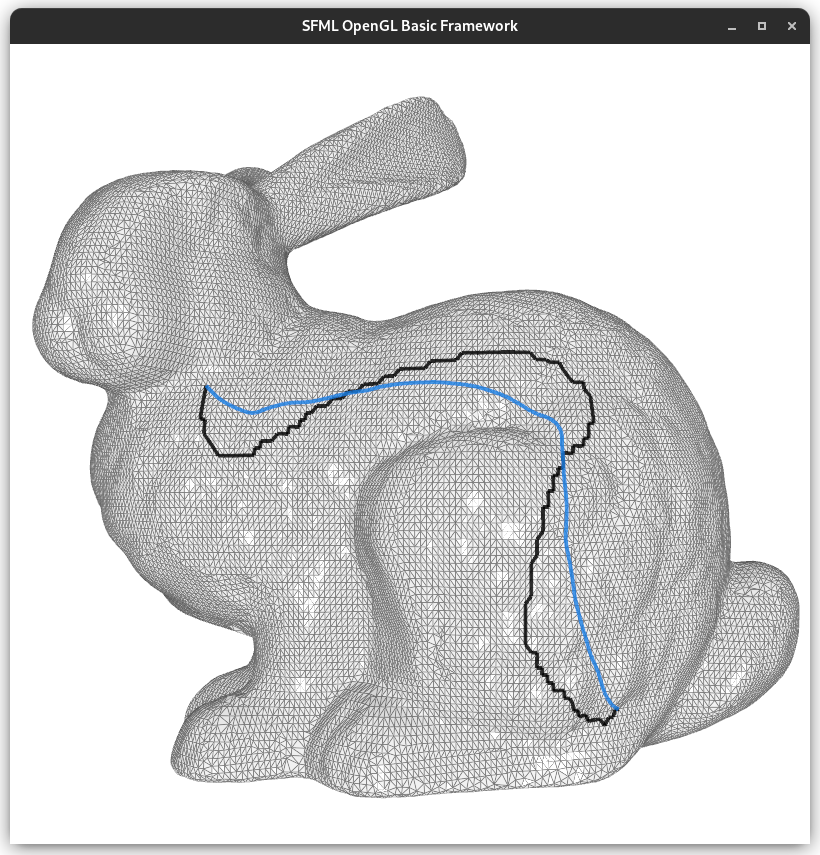
\includegraphics[width=\linewidth,trim={15px 20 15 50},clip]{images/bunny-smooth-0.5.png}
    \caption{$\sim 2000$}
  \end{subfigure}
  \begin{subfigure}[b]{0.24\linewidth}
    \centering
    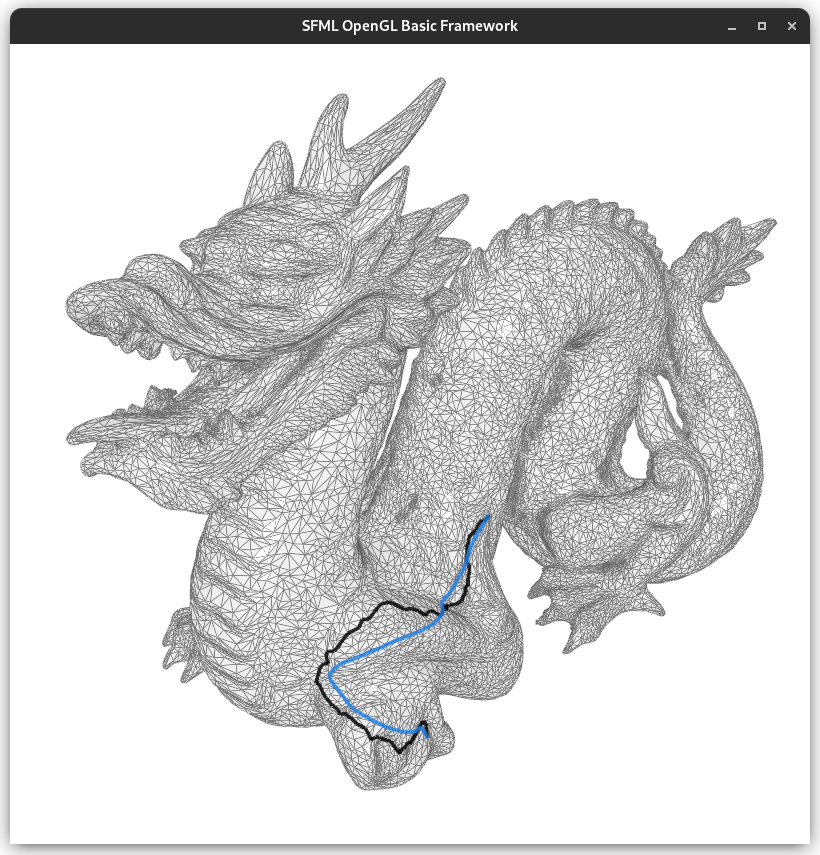
\includegraphics[width=\linewidth,trim={15px 20 15 50},clip]{images/dragon-smooth-0.5.png}
    \caption{$\sim 1500$}
  \end{subfigure}

  \begin{subfigure}[b]{0.24\linewidth}
    \centering
    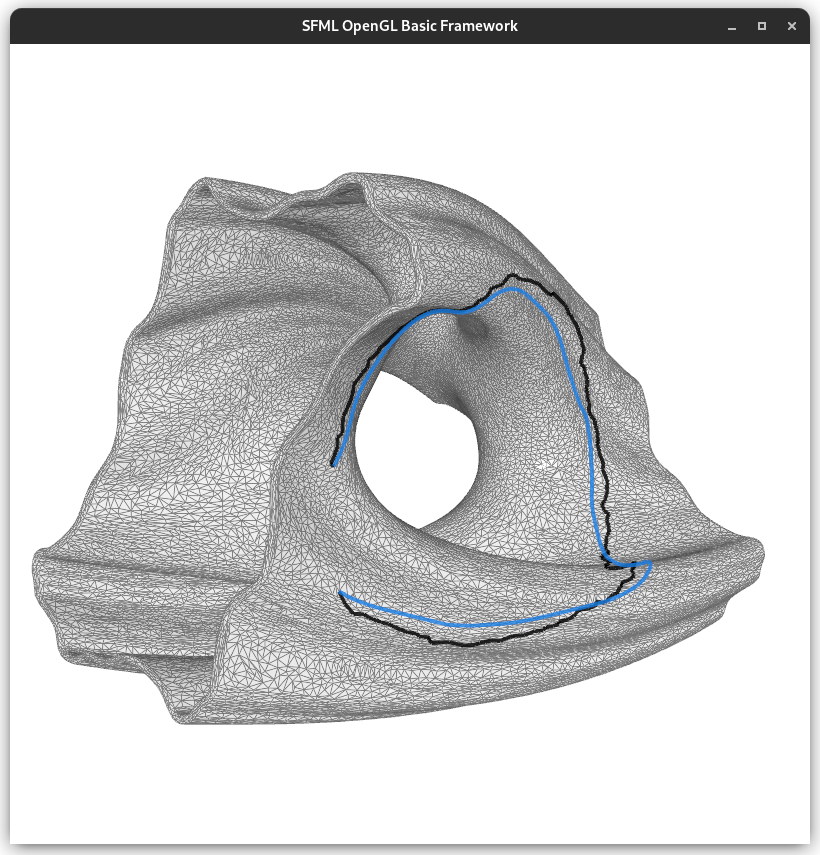
\includegraphics[width=\linewidth,trim={15px 20 15 50},clip]{images/julia-smooth-0.5.png}
    \caption{$\sim 2000$}
  \end{subfigure}
  \begin{subfigure}[b]{0.24\linewidth}
    \centering
    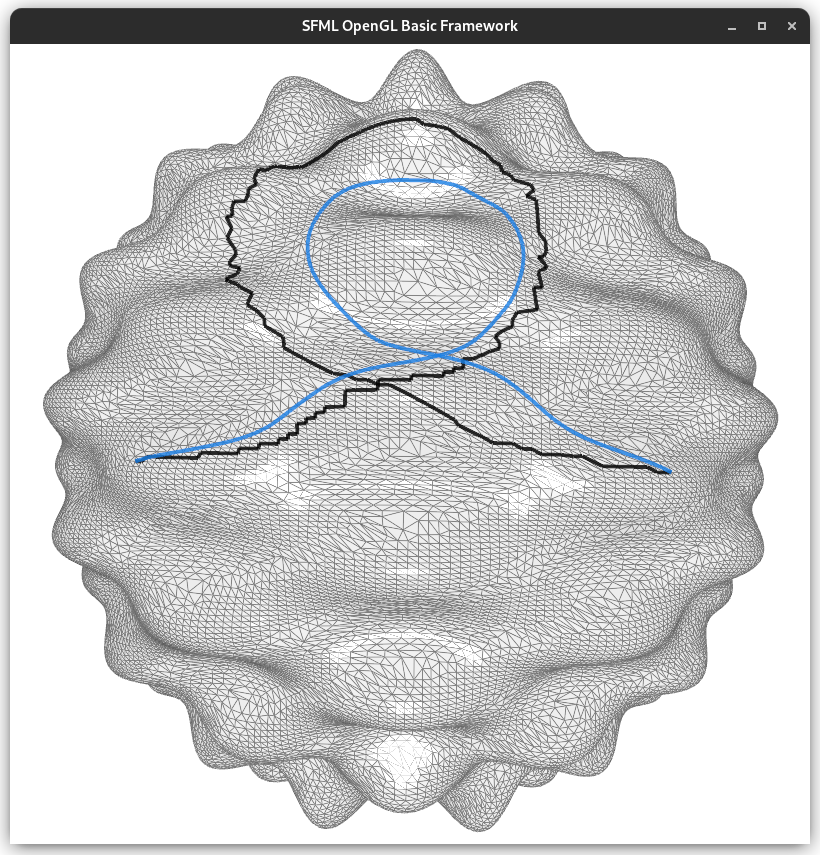
\includegraphics[width=\linewidth,trim={15px 20 15 50},clip]{images/harmonic-smooth-0.5.png}
    \caption{$\sim 4000$}
  \end{subfigure}
  \begin{subfigure}[b]{0.24\linewidth}
    \centering
    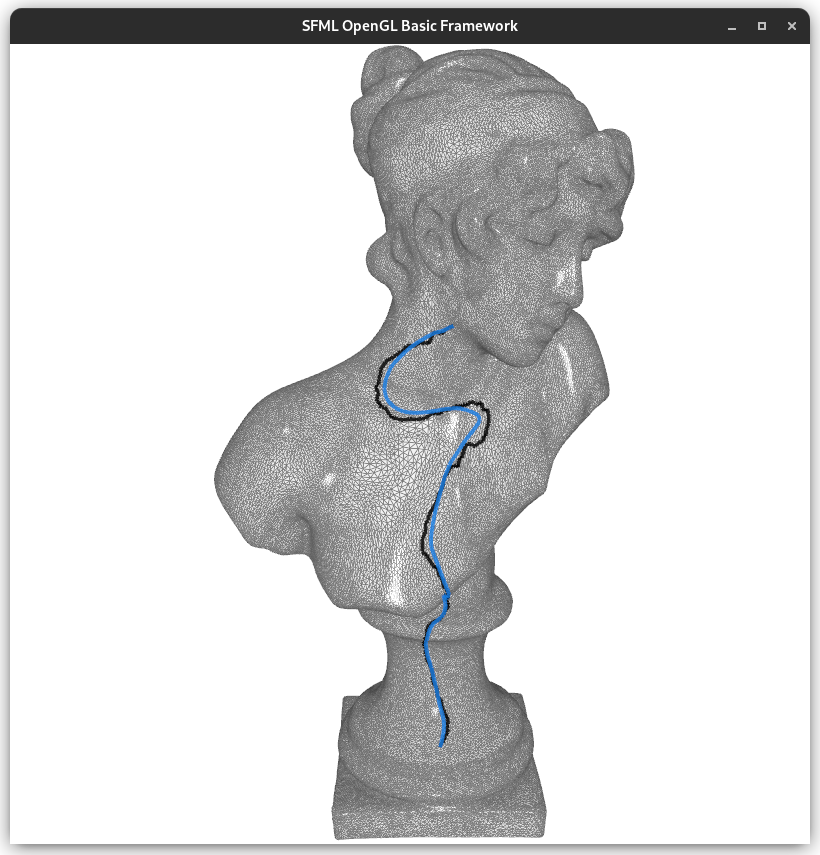
\includegraphics[width=\linewidth,trim={15px 20 15 50},clip]{images/sappho-smooth-0.5.png}
    \caption{$\sim 1500$}
  \end{subfigure}
  \begin{subfigure}[b]{0.24\linewidth}
    \centering
    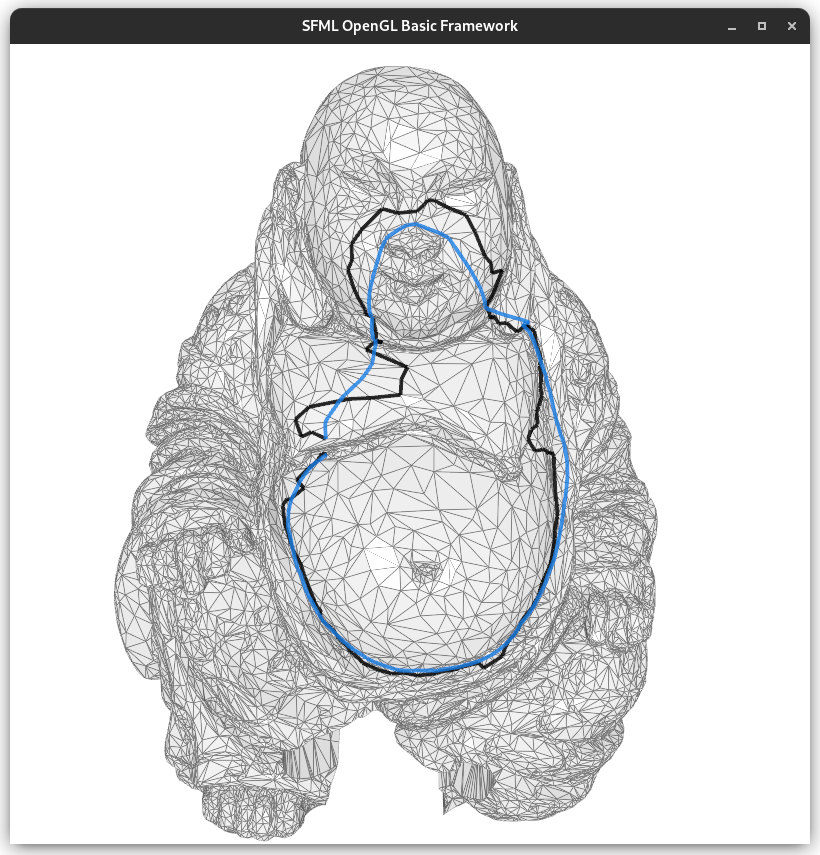
\includegraphics[width=\linewidth,trim={15px 20 15 50},clip]{images/buddha-smooth-0.5.png}
    \caption{$\sim 1000$}
  \end{subfigure}
  \caption[Qualitative Results for Smoothing with Half Scaling and Ten-Fold Stencil]{%
    \textbf{Qualitative Results for Smoothing with Half Scaling and Ten-Fold Stencil}\\
    The images show the polyhedral surfaces of the selection of models from table~\ref{tab:results-models}.
    The black curve is the initially given surface mesh curve that the smoothing algorithm transformed into the blue curve.
    The scaling value of the initialization has been set to $0.5$ and the desired geodesic curvature stencil is applied $10$ times.
    All images are labeled by the average count of iterations till convergence is reached for initial curves that are close to the depicted one.
  }
  \label{fig:results-half-scaling}
\end{figure}

\begin{figure}
  \centering
  \begin{subfigure}[b]{0.24\linewidth}
    \centering
    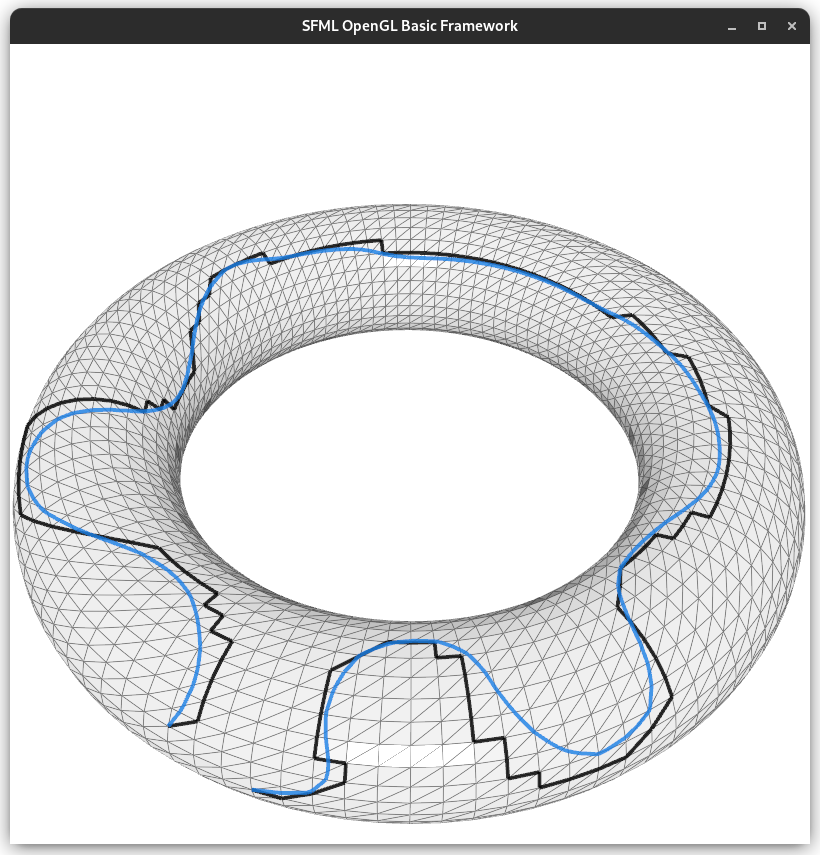
\includegraphics[width=\linewidth,trim={15px 20 15 50},clip]{images/torus-smooth-0.95.png}
    \caption{$\sim 1000$}
  \end{subfigure}
  \begin{subfigure}[b]{0.24\linewidth}
    \centering
    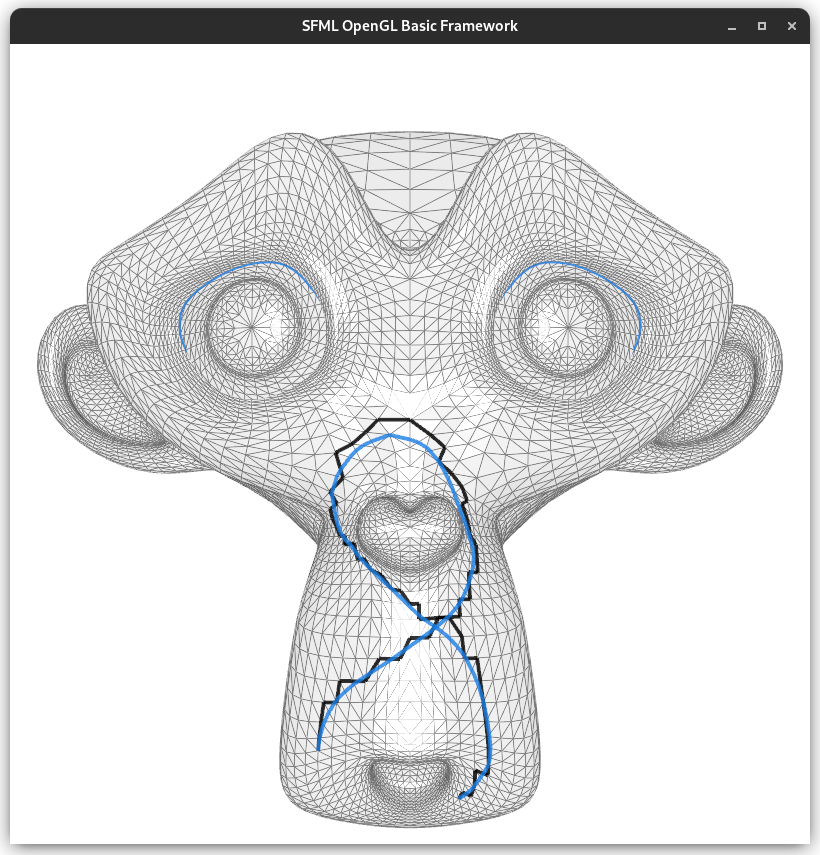
\includegraphics[width=\linewidth,trim={15px 20 15 50},clip]{images/suzanne-smooth-0.95.png}
    \caption{$\sim 400$}
  \end{subfigure}
  \begin{subfigure}[b]{0.24\linewidth}
    \centering
    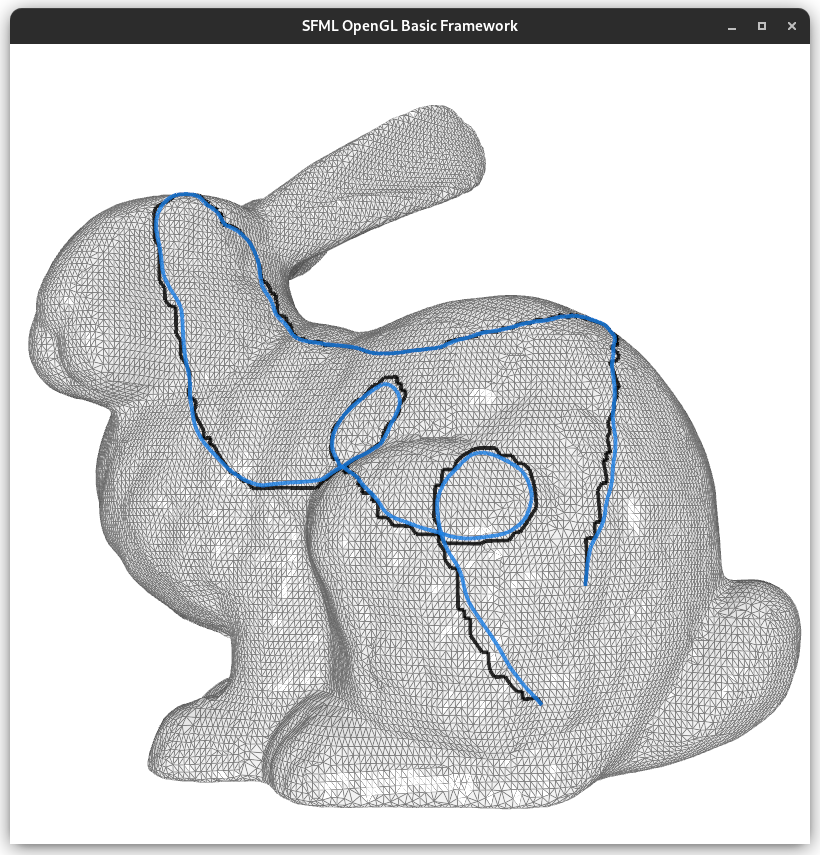
\includegraphics[width=\linewidth,trim={15px 20 15 50},clip]{images/bunny-smooth-0.95.png}
    \caption{$\sim 1000$}
  \end{subfigure}
  \begin{subfigure}[b]{0.24\linewidth}
    \centering
    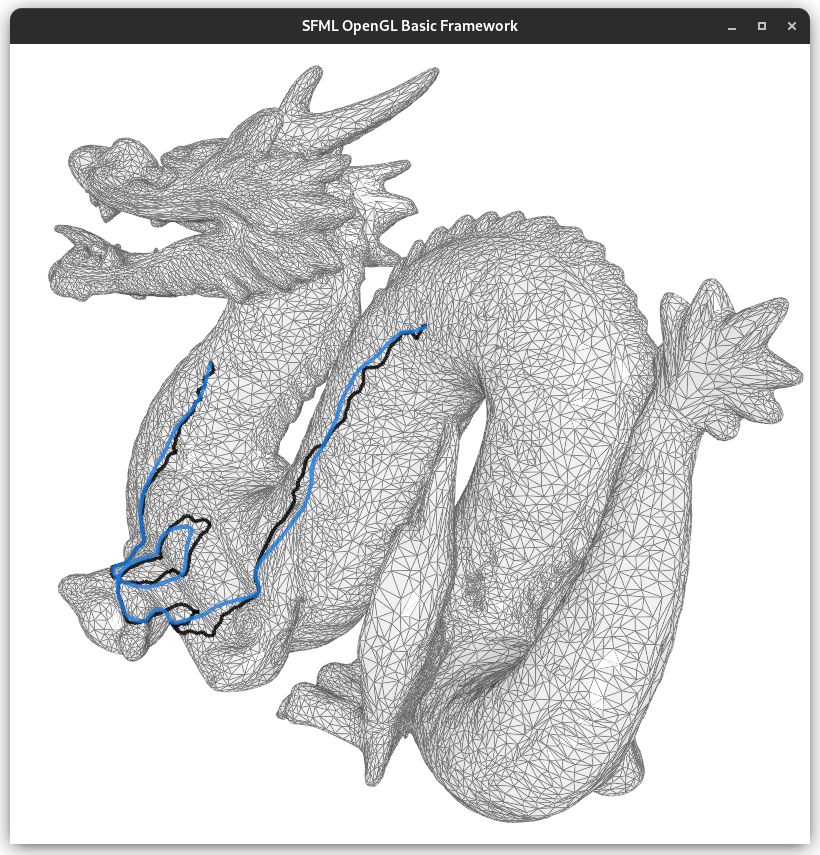
\includegraphics[width=\linewidth,trim={15px 20 15 50},clip]{images/dragon-smooth-0.95.png}
    \caption{$\sim 800$}
  \end{subfigure}

  \begin{subfigure}[b]{0.24\linewidth}
    \centering
    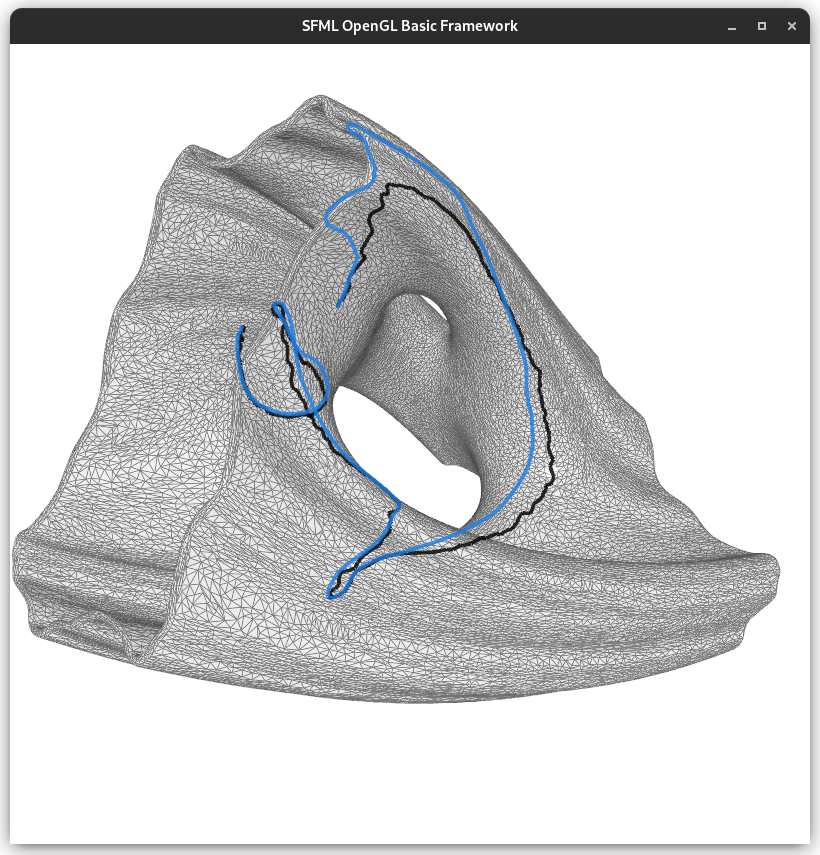
\includegraphics[width=\linewidth,trim={15px 20 15 50},clip]{images/julia-smooth-0.95.png}
    \caption{$\sim 2500$}
  \end{subfigure}
  \begin{subfigure}[b]{0.24\linewidth}
    \centering
    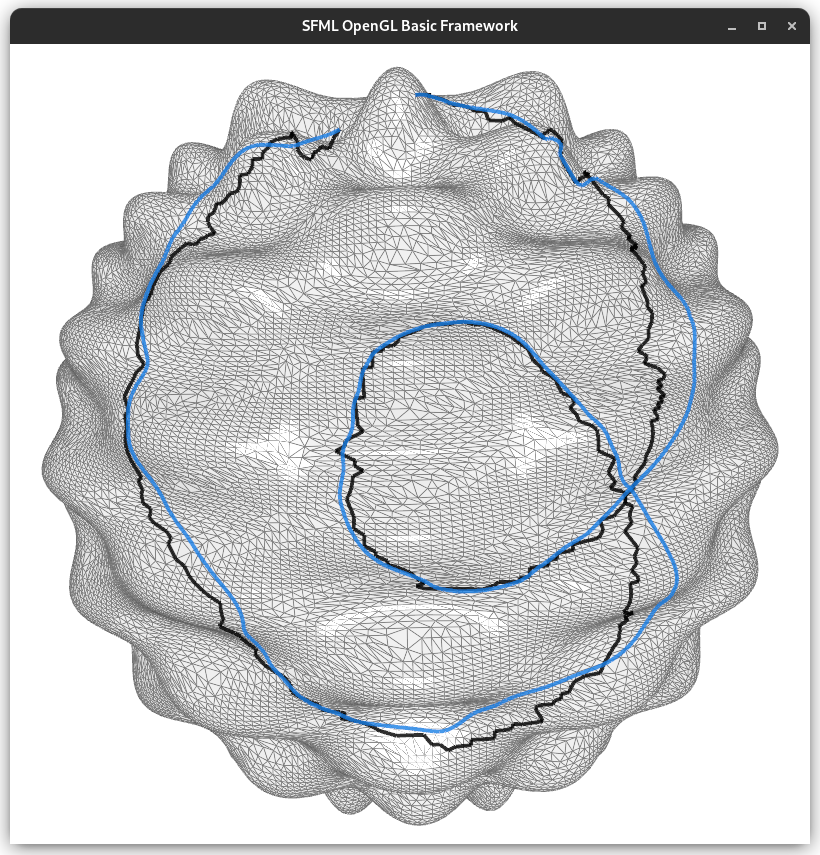
\includegraphics[width=\linewidth,trim={15px 20 15 50},clip]{images/harmonic-smooth-0.95.png}
    \caption{$\sim 3000$}
  \end{subfigure}
  \begin{subfigure}[b]{0.24\linewidth}
    \centering
    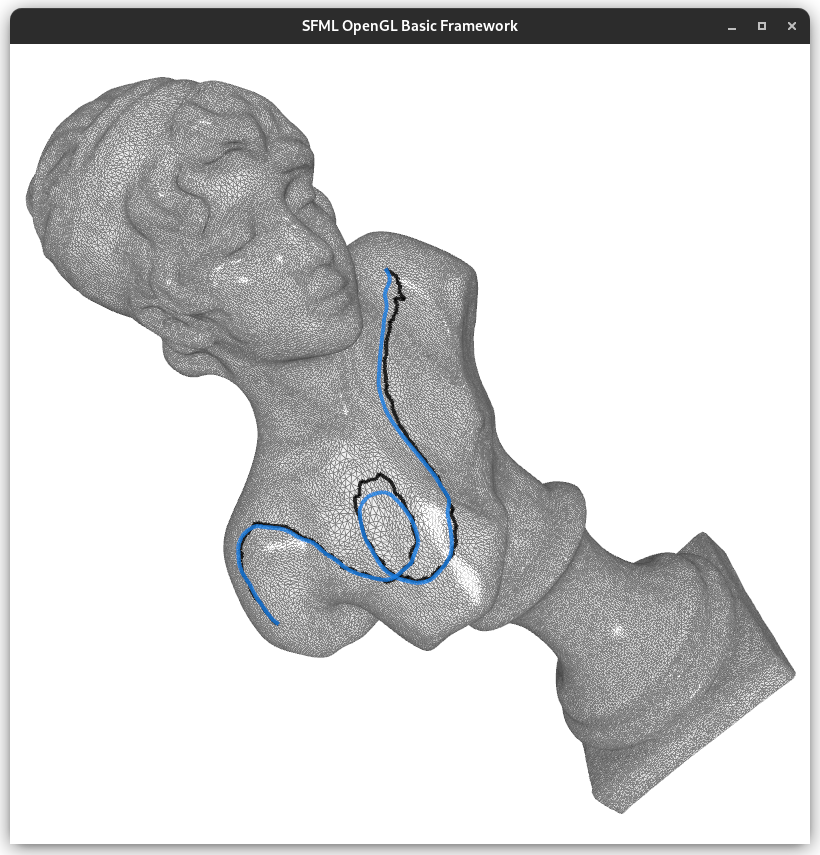
\includegraphics[width=\linewidth,trim={15px 20 15 50},clip]{images/sappho-smooth-0.95.png}
    \caption{$\sim 2000$}
  \end{subfigure}
  \begin{subfigure}[b]{0.24\linewidth}
    \centering
    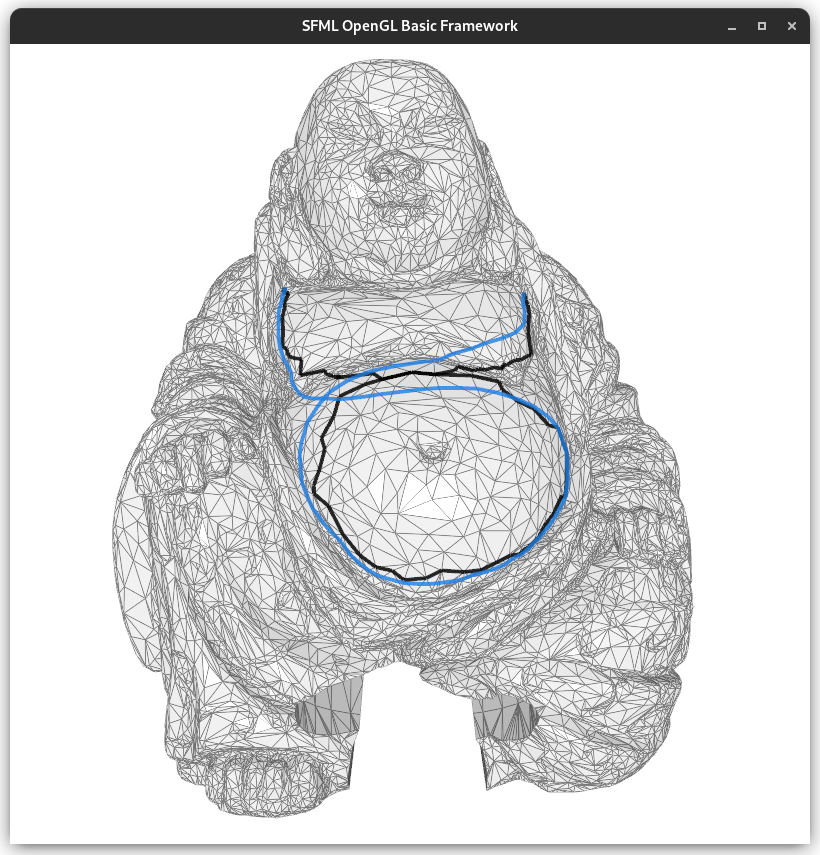
\includegraphics[width=\linewidth,trim={15px 20 15 50},clip]{images/buddha-smooth-0.95.png}
    \caption{$\sim 1200$}
  \end{subfigure}
  \caption[Qualitative Results for Smoothing with Tweaked Initialization]{%
    \textbf{Qualitative Results for Smoothing with Tweaked Initialization}\\
    The images show the polyhedral surfaces of the selection of models from table~\ref{tab:results-models}.
    The black curve is the initially given surface mesh curve that the smoothing algorithm transformed into the blue curve.
    The scaling value of the initialization has been set to $0.95$ and the desired geodesic curvature stencil is applied $5$ times.
    All images are labeled by the average count of iterations till convergence is reached for initial curves that are close to the depicted one.
  }
  \label{fig:results-tweaked}
\end{figure}

I produced curves with different scalings in an explorative manner.
In figure~\ref{fig:results-geodesics}, the generation of geodesics (with a scaling of $0$) is robust and produces very smooth curves under any cicrumstances since every iteration shortens the overall length of the curve.
% This scaling leads to convergence under any circumstances.
Yet, given the definition of geodesics, the curvature mainly depends on start and end points of the initially provided curve and hence does not guarantee a close distance to the initially provided curve.
In figure~\ref{fig:results-no-scaling}, the smoothing procedure with a scaling of $1$ produces smooth curves which are very close the initially provided curve.
% in figure 5.1, yet
% Unfortunately, it is not robust.
Unfortunately, a curvature-based smooting with a scaling of $1$ might lead to the expansion of the surface mesh curve.
Due to the lack of the strict contraction property, contrary to the previous case, this might not lead to convergence under any circumstances.

Figure~\ref{fig:results-half-scaling} illustrates the use of a scaling of $0.5$ as a middle ground between the two extreme scalings depicted before.
Based on this, I approximate a scaling value which provides the best trade-off between smoothness and closeness to the initially drawn curve, tackling both aforementioned problems.
The results use a scaling of $0.95$ and are depicted in figure~\ref{fig:results-tweaked}.

Furthermore, figure~\ref{fig:results-geodesic-iterations} shows different iterations of geodesic smoothing applied to an initially given surface mesh curve on a sphere-approximating polyhedral surface.
It becomes clear that the first few iterations of the geodesic-based smoothing already provide a certain kind of smoothing.
Instead of waiting for convergence, smoothing can also be carried out by applying only apply small number of geodesic iterations to an initial curve.

\begin{figure}
  \centering
  \begin{subfigure}[b]{0.24\linewidth}
    \centering
    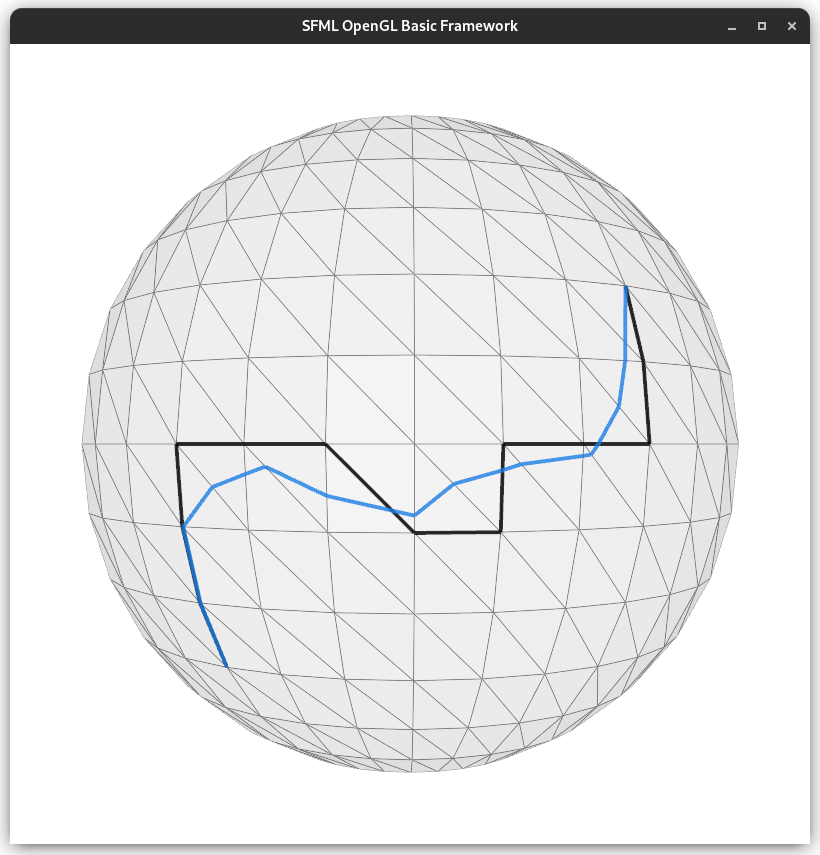
\includegraphics[width=\linewidth,trim={15px 20 15 50},clip]{images/sphere-geodesic-1-iteration-1.png}
    \caption{1}
  \end{subfigure}
  \begin{subfigure}[b]{0.24\linewidth}
    \centering
    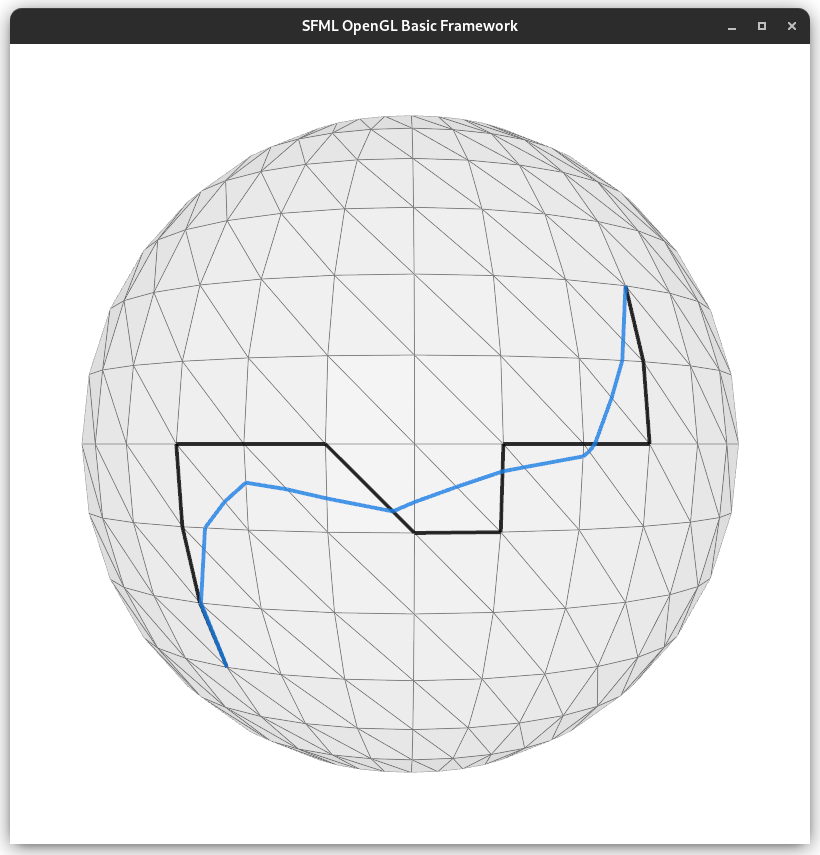
\includegraphics[width=\linewidth,trim={15px 20 15 50},clip]{images/sphere-geodesic-1-iteration-2.png}
    \caption{2}
  \end{subfigure}
  \begin{subfigure}[b]{0.24\linewidth}
    \centering
    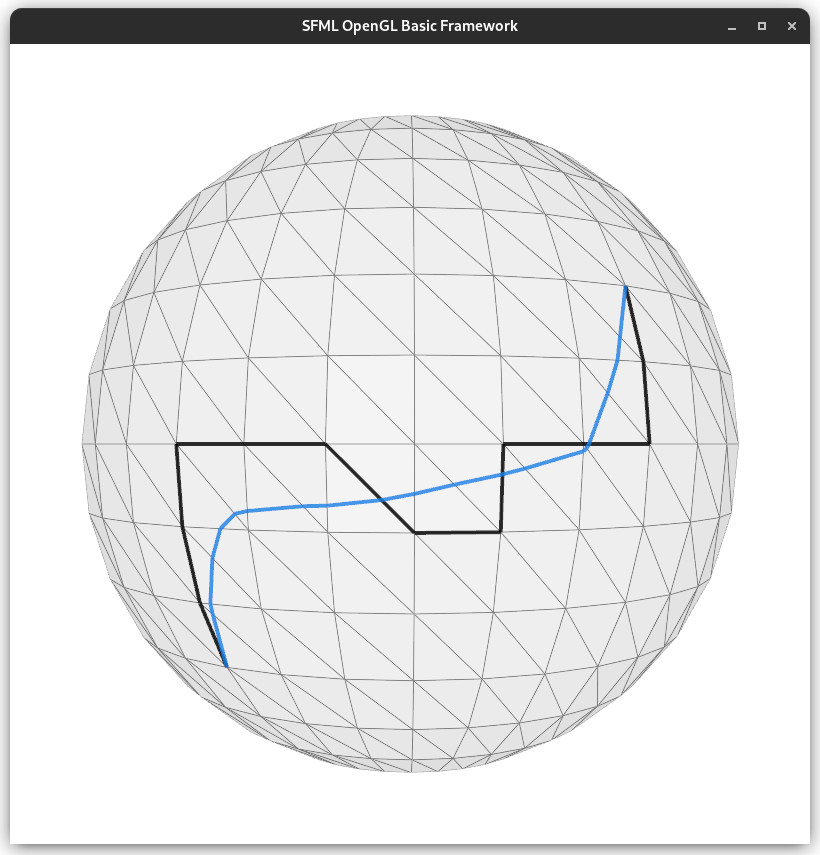
\includegraphics[width=\linewidth,trim={15px 20 15 50},clip]{images/sphere-geodesic-1-iteration-4.png}
    \caption{4}
  \end{subfigure}
  \begin{subfigure}[b]{0.24\linewidth}
    \centering
    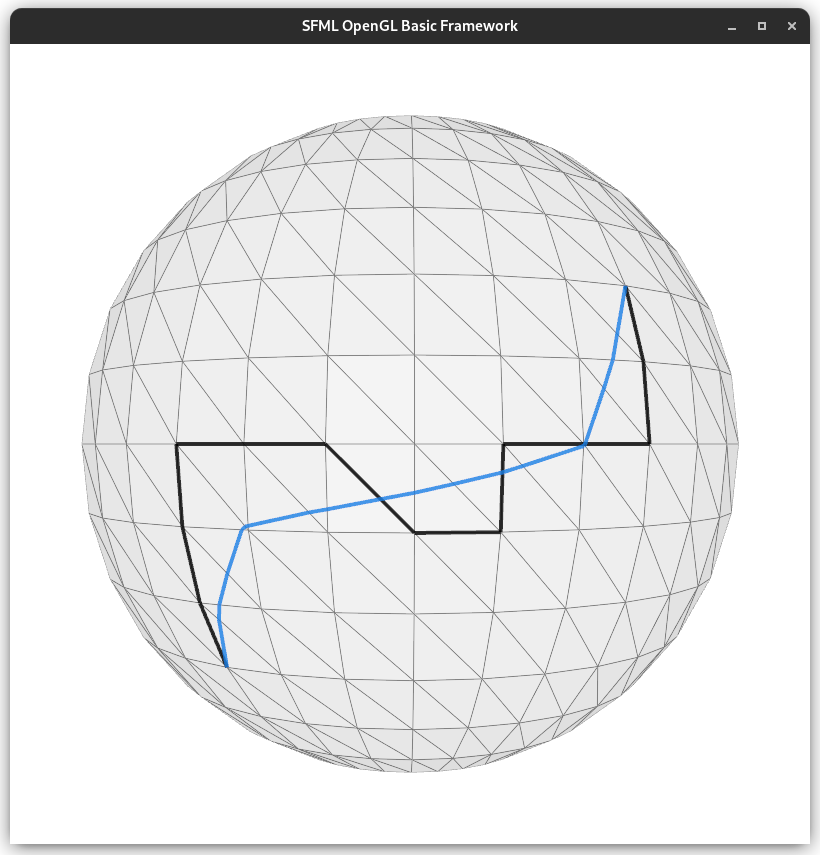
\includegraphics[width=\linewidth,trim={15px 20 15 50},clip]{images/sphere-geodesic-1-iteration-8.png}
    \caption{8}
  \end{subfigure}
  \begin{subfigure}[b]{0.24\linewidth}
    \centering
    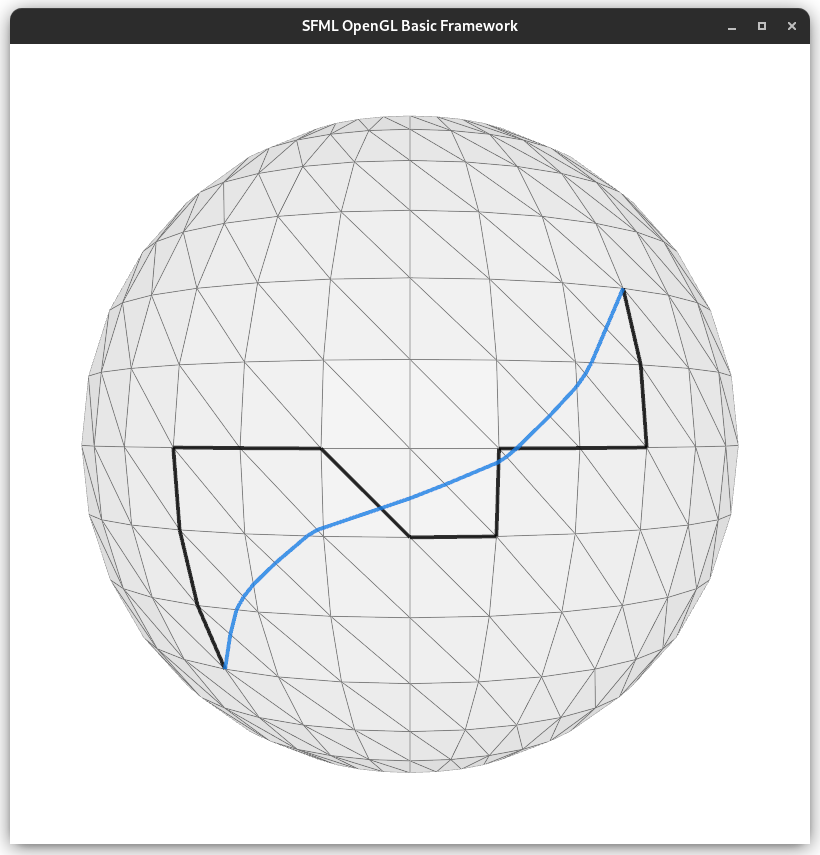
\includegraphics[width=\linewidth,trim={15px 20 15 50},clip]{images/sphere-geodesic-1-iteration-16.png}
    \caption{16}
  \end{subfigure}
  \begin{subfigure}[b]{0.24\linewidth}
    \centering
    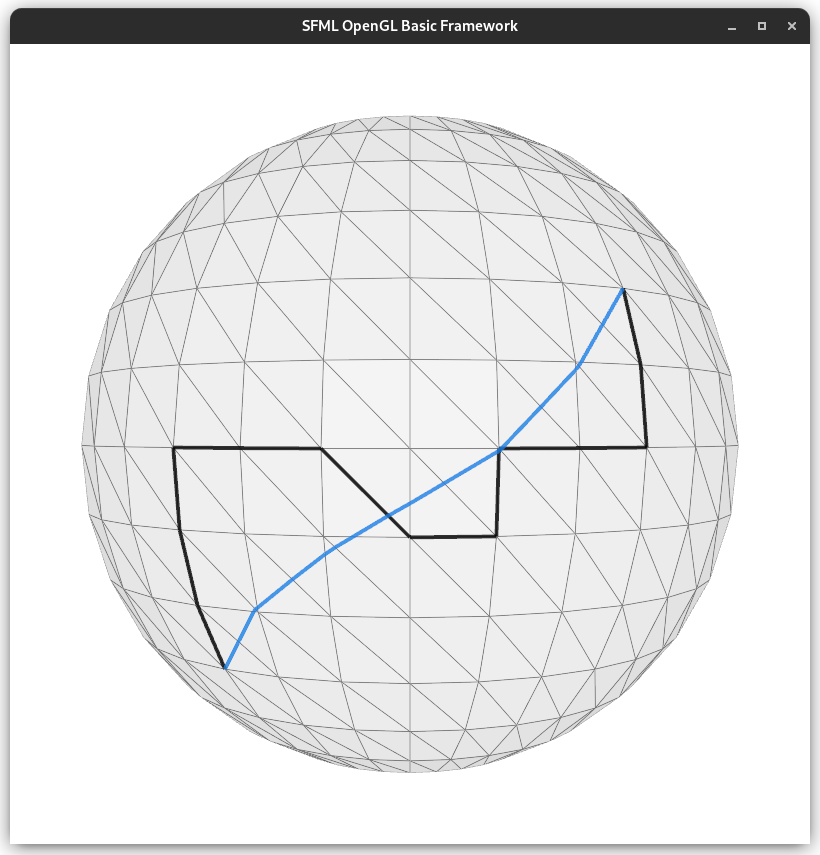
\includegraphics[width=\linewidth,trim={15px 20 15 50},clip]{images/sphere-geodesic-1-iteration-32.png}
    \caption{32}
  \end{subfigure}
  \begin{subfigure}[b]{0.24\linewidth}
    \centering
    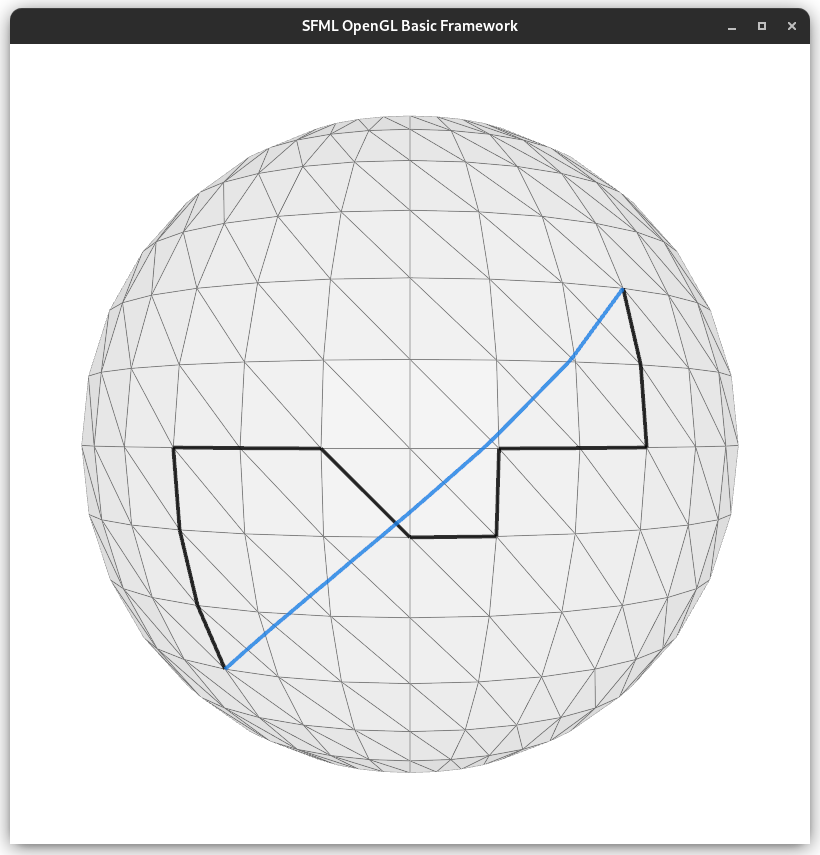
\includegraphics[width=\linewidth,trim={15px 20 15 50},clip]{images/sphere-geodesic-1-iteration-64.png}
    \caption{64}
  \end{subfigure}
  \caption[Qualitative Results for Geodesics Iterations]{%
    \textbf{Qualitative Results for Geodesics Iterations}\\
    The images show a polyhedral surface that approximates a sphere with an initially given surface mesh curve depicted in black.
    The blue curve represents the result of the geodesics generation after a number of iterations that is given as label for each image.
    In this example, after $64$ iterations the initial curve has been converged to the geodesic.
  }
  \label{fig:results-geodesic-iterations}
\end{figure}

% \paragraph{Smoothing via Geodesics Iterations}\hfill\\
% After a finite amount of iterations for geodesics generations the curve is already smooth.

% section evaluation (end)
\end{document}
